\documentclass[10pt,border=2pt]{standalone}
\usepackage[T1]{fontenc}
\usepackage{lmodern}
\usepackage{pgfplots}
\pgfplotsset{compat=1.18}
\definecolor{convexblue}{HTML}{0072B2}
\definecolor{concaveorange}{HTML}{D55E00}
\begin{document}
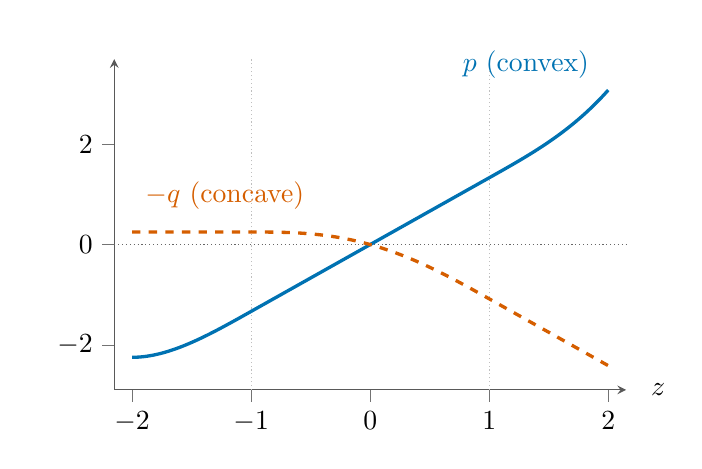
\begin{tikzpicture}
\path[use as bounding box] (-1.1,-0.65) rectangle (7.1,4.6);
\begin{axis}[
  scale only axis,width=6.5cm,height=4.2cm,
  at={(0,0)},anchor=south west,
  xmin=-2.15,xmax=2.15,xtick={-2,-1,0,1,2},
  ymin=-2.9,ymax=3.7,ytick={-2,0,2},
  axis lines=left,axis line style={black!65},
  tick align=outside,tick style={black!55},
  xlabel={$z$},xlabel style={at={(axis description cs:1.03,0)},anchor=west},
  label style={font=\normalsize},tick label style={font=\normalsize},
  clip=false,
]
\addplot[black!60,densely dotted,thin] coordinates {(-2.15,0) (2.15,0)};
\addplot[black!25,densely dotted,thin] coordinates {(-1,-2.9) (-1,3.7)};
\addplot[black!25,densely dotted,thin] coordinates {(1,-2.9) (1,3.7)};
\addplot[convexblue,very thick,domain=-2:2,samples=241]
  {x < -1 ? x^4/12-x^2/2+2*x/3-1/4 : (x > 1 ? x^4/12-x^2/2+2*x-1/4 : 4*x/3)};
\addplot[concaveorange,very thick,dashed,domain=-2:2,samples=241]
  {x < -1 ? 1/4 : (x > 1 ? -4*x/3+1/4 : x^4/12-x^2/2-2*x/3)};
\node[convexblue,anchor=south east] at (axis cs:1.92,3.13) {$p$ (convex)};
\node[concaveorange,anchor=south west] at (axis cs:-1.97,0.5) {$-q$ (concave)};
\end{axis}
\end{tikzpicture}
\end{document}
